\vspace{.1in}
\section{Windowing} \label{sec:tern-window}

Server programs present two challenges for \tern.  First, they 
are more exposed to
timing nondeterminism than batch programs because their inputs
(client requests) arrive nondeterministically.  Second, they often run
continuously, making their schedules too specific to reuse.

%% \begin{figure}[t]
%% \begin{center}
%% 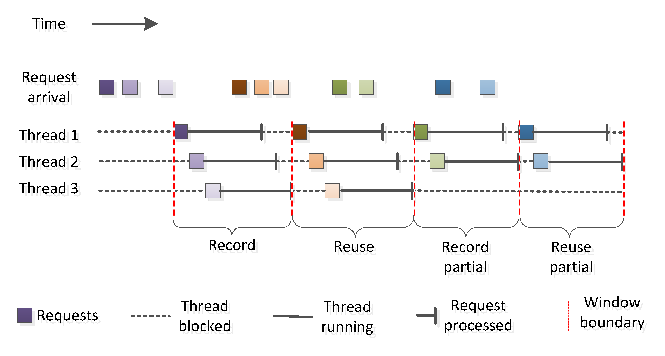
\includegraphics[width=0.47\textwidth]{figures/window-idea.eps}
%% \end{center}
%% \caption{\emph{Windowing idea.}}
%% \label{fig:window-idea}
%% \end{figure}

\tern addresses these challenges using a simple idea called
\emph{windowing}.  Our insight is that server programs tend to return to the
same quiescent states.  Thus, instead of processing requests as they
arrive, \tern breaks a continuous request stream down to windows of
requests.  Within each window, it admits requests only at fixed points in
the current schedule.  If no requests arrive at an admission point for a
predefined timeout, \tern simply proceeds with the partial window.  While a
window is running, \tern buffers newly arrived requests so that they do not
interfere with the running window.  With this approach, \tern can memoize
and reuse schedules across (possibly partial) windows.
%% Figure~\ref{fig:window-idea} illustrates this idea applied to a window
%% with four threads.  (Window size is configurable and defaults to the
%% number of CPUs.)  
The cost of windowing is that it may reduce concurrency
and degrade server throughput and speed.  However, our experiments show
that this cost is reasonable and justified by the gain in determinism
and stability.

To buffer requests, \tern needs to know when a server receives a request
and when it is done processing the request.  Inferring these task
boundaries based on thread creation and exit is unreliable because server
programs frequently use thread pools.  Thus, \tern currently lets
developers annotate these boundaries using \vv{begin\_task()} and
\vv{end\_task()}.  Manually locating task boundaries is often easy: a
request tends to begin after an \vv{accept()} of a client connection and ends
after the server sends out a reply.

\para{Exposing hidden states.}  The assumption of windowing is that a
server program returns to the same state when it quiesces.  However, in
practice, server states evolve over time.  For instance, when Apache first
serves a page, it may load the page from disk and cache it in memory.
When this page is requested again, Apache can serve it directly from its
cache.

These state changes may affect schedules.  In the example above, Apache
will perform different synchronizations for the two runs.  Thus, for
\tern to accurately select a schedule to reuse, it must know the hidden
states that affect schedules.  Currently \tern lets developers annotate
such hidden states using \vv{symbolic()}.  Doing so is often
straightforward.  For instance, we inserted a \vv{symbolic()} call to mark
the return of Apache's \vv{cache\_find()} as symbolic.

Exposing hidden states may not always be easy.  We thus created a
technique to tolerate missed \vv{symbolic()} annotations.  The basic idea
is to store backup schedules under the same set of input constraints to
tolerate annotation inaccuracy.  For instance, suppose a \vv{symbolic()}
had not been missed, \tern would have memoized two different
constraint-schedule tuples $\langle C_1, S_1 \rangle$ and $\langle C_2,
S_2 \rangle$.  However, because of the missed annotation, \tern missed the
corresponding constraints, wrongly collapsing $C_1$ and $C_2$ into the
same set $C$.  Now the two original tuples become $\langle C, S_1 \rangle$
and $\langle C, S_2 \rangle$, which appear redundant.  Instead of
discarding one of these seemingly redundant schedules, \tern will store both
schedules with the same set of constraints.  To select between these
schedules, \tern can select the one with higher reuse rate, which likely
matches the hidden state of the program.

